\makeatletter                                                   
\def\input@path{{../}}                                          
\makeatother                                                    
\documentclass[../main.tex]{subfiles}                           
\begin{document}                                                
\chapter{Computational Results}
\label{ch:res}
This chapter will present the results from several experiments leading us to the experiments of a final composition of our ALNS model. \par 
We start by explaining the experimental setup of our testing in \cref{sec:setup}. Then we will explain the instances we used in our experiments in \cref{sec:ins}. \par
\Cref{sec:iniRes} contain the initial experiments of our model that lead us to the final composition of our model. 
The first part, \cref{sec:evalW}, starts by testing the wild algorithm from \cref{sec:wild} and it finds that the wild algorithm outperforms a random restart and not using any escape algorithm.
Then in \cref{sec:evalH1} we rank the heuristics performance and do ANOVA(III) and multiple linear regressions of the heuristics described in \cref{ch:appr}. 
We find here that three heuristics have a significant positive influence on the result, the remove random and insert first first algorithm from \cref{sec:rand}, the remove worst and insert greedy heuristic from \cref{sec:greedy}, and the remove similar and insert regret-3 heuristic from \cref{sec:shaw}. \par
We continue our initial experiments in \cref{sec:evalH2} with extended ANOVA(III), multiple linear regression models and pairwise t-tests to evaluate if combining the not significant heuristics with the significant ones from \cref{sec:evalH1}, can have a significant positive impact on the result.
Here we find that the remove non-clustered and insert clustered heuristic from \cref{sec:clust} has a singificant positive influence on the best solution found. 
We also find that the swap first fit heuristic from \cref{sec:swap} has no significant influence on the result. \par
In \cref{sec:finComp} we present the final composition of our model which contain the heuristics mentioned above aswell as the wild algorithm.\par
The final part of this chapter \cref{sec:evalFin} contains the evaluation of our final model composition and compares the results from the mathematical model from \cref{ch:mm} with the results of our model. It also presents an evaluation of the performance of the included heuristics.
The results show a robust and efficient alorithm.

\section{Experimental Setup}
\label{sec:setup}
In this section we describe the technical setup of the experiments aswell as the Analytical setup of our eperiments.
\subsubsection{Technical Setup}
The computational experiments in this paper are run on a 64-bit Ubuntu 18.04 computer with a 1.8 Ghz quad core i7-8550u processor and 16GB RAM. 
In \cref{sec:ins} we will describe an instance generator and this was implemented using Java \citep{java}.
The mathematical model from \cref{ch:mm} is setup in AMPL \citep{ampl}, using the Gurobi solver \citep{gurobi}.  
We used Java \citep{java} to write the program to run the solution method from \cref{ch:appr}.
The ANOVA(III), multiple linear regressions and t-tests are performed in Matlab \citep{matlab}.

\subsubsection{Analytics Setup}
To test our model from \ref{ch:appr} we generated five instance sets, each containing five instances of different sizes, totally 25 instance. 
Each instance set is described in \cref{sec:ins}.
While testing the algorithm from \cref{sec:wild}, we used one of these instance sets, ie. 5 instances. 
All tests were run 10 times and results are given as an average and best objective value over the 10 runs aswell as an average running time.
To analyse the performance of each of the heuristics in \cref{sec:evalH1} and \cref{sec:evalH2}, 5 reasonably sized instances (80 orders) were solved 10 times using each of the $2^7 = 128$ combinations of heuristics.
Here we also try to determine which of the heuristics influence the result by performing several statistical experiements, including ANOVA (III) and multiple linear regression analysis, and pairwise t-tests.
For all statistical experiments in this paper we have used a $95\%$ confidence interval.
After the analysis of the heuristics, a final composition was chosen for further testing in \cref{sec:evalFin}.
Here we then compared the performance of the final composition with solutions found by the mathematical model. 
We also present figures which show the performance of our selected heuristics in arbitrarily selected runs.

\section{Instances}
\label{sec:ins}
Many instance generators have been created for pickup and delivery problems. \cite{hemmati14} made an instance generator for tramp shipping routing and scheduling problems.
Our instance generator was created based on real world data from an anonumous customer of 4flow.
In the following, we will describe how we designed the generator and how we generated the instances used in the analytical part of this thesis.

\subsection{Generate Instances based on real world data}
\label{sec:data}
The 4flow data gives information about the number of orders $|N|$, locations $|L|$, factories $|F|$. 
The amount of vehicles $|V|$ are selected based on 4flow data and are in the bound between $|N|/2 \leq |V| \leq 2/3 |N|$.
We give $|N|, |V|, |L|, |F|$ as input to the generator.\par
In addition the data from 4flow gave us information about the size of a vehicle and its compatabilities. 
Some vehicles might have cooling possibilities, some orders might require special equipment for transport, (like breakable or explosive goods) or there might be equipment required at the pickup or delivery location (like f.eks. a crane to unload goods).
We refer to these capabilities as a \emph{vehicle requirement}.
Other information aquired by the data was travel distances and cost structure.

\par
In the following we refer to the mathematical symbols from \ref{ch:mm}. To keep the instances feasible but still as realistic as possbile it makes sense to limit the data to ranges or predesigned patterns.
Our data was generated based on the following possibilities:
\begin{itemize}
    \item Orders are assigned to pickup and delivery locations randomly. Orders assigned to the same location are given the same stop $L_s$.
    \item Each delivery location is independently assigned to a factory at random $N_f$.
    \item $5\%$ of each order and location were on average given a vehicle requirement. This will decide which vehicle can pickup which order, $N^P_v$ and $N^D_v$.
    \item We let the vehicles types be split up in 3 different vehicle types, small, medium, large, each with expected capacities and capabilities.
        \begin{itemize}
            \item Large vehicle: slow speed vehicle compatible with all locations and orders, with $Q^{kg}_v=24k$ and $Q^{vol}_v=102$.
            \item Medium vehicle: medium speed vehicle and compatible with all locations but not orders with vehicle requirements, with $Q^{kg}_v=18k$ and $Q^{vol}_v=71$.
            \item Small vehicle: fast speed vehicle, not compatible with any vehicle requirements, with $Q^{kg}_v=12k$ and $Q^{vol}_v=55$.
        \end{itemize}
    \item The distances $d_{ij}$ are euclidian distances between the randomly generated points described in the next paragraph.
    \item The travel time $T_{ijv}$ were scaled with $60\%$ of the travel distance, added with a random variation of $+/- 10\%$ of the travel distance. The travel time also depends on the speed of the vehicle mentioned above. Slow speed vehicles had a $5\%$ increase in travel time while medium speed had a $2.5\%$ increase and fast speed vehicles had no increase in travel time.
    \item The cost matrices $C^{km}_{v\alpha\beta}$, $C^{kg}_{v\alpha\beta}$, $C^{fix}_{v\alpha\beta}$ were based on a real 4flow cost matrix, scaled to the size of the instance and to the size of the vehicle.  
    \item The cost of not transporting an order $C_i$ was set to a minimum lower bound (the most expensive transport) and scaled based on the weight, volume and distance of the order.
    \item The stop costs $C^{stop}_{vi}$ were calculated relative to the size of the vehicle and the cost data from 4flow.
    \item Time windows $[\underline{T_{ip}},\overline{T_{ip}}]$  were generated randomly based on typical factory opening hours. Meaning, one to two timewindows per day, and three to sevem days per week scaled based on the instance size. 
\end{itemize}

\subsubsection{Random locations based on real geographical data}
Most of 4flow's customers are based either in Germany or in Europe. 
To make the instance generator as realistic as possible we have decided to split the instances into 3 geographical types; 
European, German and uniform geographically distributed locations.
We made 2 maps based on real scale approximations of geographical data from National Geographics, in km.
To simplify we have sticked to geographical points with an eliptic uniformly distributed area surrounding the point to represent a country or a city.
\cref{fig:areas} illustrates the areas of possible locations used in the generator. 
Larger elipses are more likely to be selected by the generator than smaller elipses.
\begin{figure}
\centering
    \caption{Area of random point generation}
    \begin{subfigure}[b]{0.3\textwidth}
        \centering
        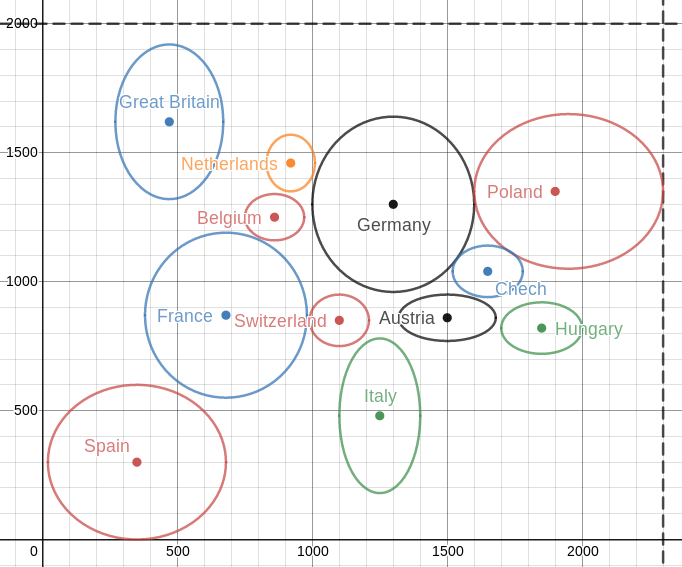
\includegraphics[width=\textwidth]{europe_coordinates}
        \caption{Europe}
        \label{fig:eur}
    \end{subfigure}
    \hfill
    \begin{subfigure}[b]{0.3\textwidth}
        \centering
        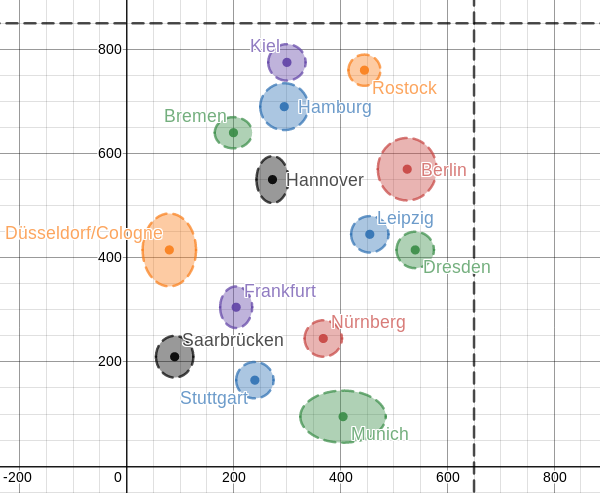
\includegraphics[width=\textwidth]{germany_coordinates}
        \caption{Germany}
        \label{fig:ger}
    \end{subfigure}
    \hfill
    \begin{subfigure}[b]{0.3\textwidth}
        \centering
        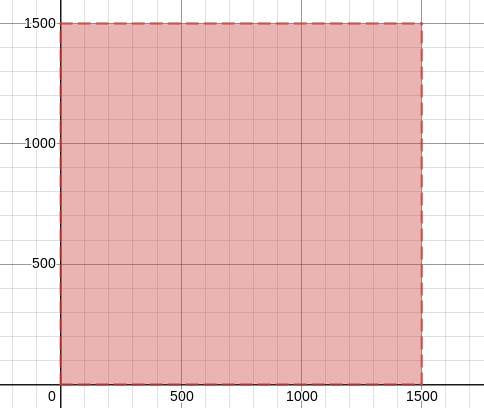
\includegraphics[width=\textwidth]{uniform_coordinates}
        \caption{Uniform}
        \label{fig:uni}
    \end{subfigure}
    \label{fig:areas}
    \caption*{For Europe and Germany, shaded areas indicate a possible location generation. Larger areas are more likely to generate a point. Uniform means location points were generated using a uniform distribution within the greyed area.}
\end{figure}

For the selected elipse a point was selected within the elipse at random with a uniform distribution.
For \cref{fig:uni} points were generated at random within the limits shown.
From our 5 instance sets, two were generated using \cref{fig:eur}, two with \cref{fig:ger} and one with the uniform distribution from \cref{fig:uni}. 
If a point belong in the same factory as a previously generated point, that point was generated within a reasonable radius of three kilometer.

\subsection{Generated Instances}
\label{sec:geni}
For testing our algorithm, 5 instance sets of each 5 instances of varying sizes were generated. 
We have numbered the sets as follows:
\begin{itemize}
    \item Set 1 and Set 2 are generated based on the European map from \cref{fig:eur}.
    \item Set 3 and Set 4 are generated on the german map from \cref{fig:ger}.
    \item Set 5 is generated on the uniform distribution from \cref{fig:uni}.
\end{itemize}

Each instance set contain representative instance sizes of our problem based on data from 4flow, $4, 12, 35, 80$ and $150$ orders using respectively $3, 7, 20, 45$ and $80$ vehicles and containing $7, 9, 22, 45$ and $85$ locations.  
The sizes of the instances and the instance set number are shown for each result presented in the following sections.

\section{Initial Results}
\label{sec:iniRes}
In this section we present the results and observations from our initial experiments. 
This data lead us to the final composition of our model.
We have done this in 3 parts. \Cref{sec:evalw} contain the evaluation of our wild escape algorithm. Then follows \cref{sec:evalH1} which is the initial evaluation of the heuristics. Finally \cref{sec:evalH2} contain the further evaluation of the heuristics.
Afterwards, in \cref{sec:finComp}, we will present the final composition of the model.

\subsection{Evaluation of the wild algorithm}
\label{sec:evalW}
To help our algorithm escape from a local optimum, we designed a wild algorithm described in section \cref{sec:wild}. 
To evaluate the implementation of this algorithm we have decided to compare the result of running the complete model from \cref{ch:appr} including all heuristics, with three different modifications.
We ran all modifications on instance Set 1.
First modification was that we ran the algorithm without any escape algorithm, refered to as \emph{no escape}.
Secondly we ran the algorithm with a modification that resets the algorithm each time we get stuck in a local optimum and then start from a new random solution, refered to as \emph{random reset}.
Lastly, we ran our algorithm with our \emph{wild escape algorithm}.
Comparing these three options towards eachother will help us evaluate if our wild algorithm is helping us in general and see if our wild algorithm is different than doing a reset and just starting from a new solution somewhere.

\subsubsection{Results of escape modifications}
We ran our algorithm 10x3 times, ten for each escape adjustment, on instance set 1 from \cref{sec:ins}.
We modified our escape algorithm on this run to ignore if a best solution is found while moving from one neighbourhood to the next. 
This way the extra iterations explained in \cref{sec:wild}, does not give any unfair advantage to our wild escape algorithm. We will simply be moving from one neighbourhood to the next without checking if we find a better solution on the way.
\par
The result from running our algorithm with these three adjustments are summarized in \cref{tab:wildComp}.
It shows the objective values found on average during each of the 10 runs, the best solution found overall and the average running time, for each escape adjustment.
\begin{table}
    \centering
    \caption{ALNS with all heuristics using 3 different reset algorithms}
    \begin{adjustbox}{width=\columnwidth,center}
            \begin{tabular}{|ccc|c|ccc|ccc|ccc|}
            \hline
                        &           &           &                   & \multicolumn{3}{c|}{Average Objective}        & \multicolumn{3}{c|}{Best Objective}            & \multicolumn{3}{c|}{Running time (sec)}   \\ 
                        &           &           & Initial           & No            & Random        & Wild          & No            & Random        & Wild          & No        & Random    & Wild      \\     
                \#Ord   & \#Veh     & \#Loc     & objective         & escape        & reset         & escape        & escape        & reset         & escape        & escape    & reset     & escape    \\
            \hline
                4       & 3         & 7         & $609\,680.3$      & $3\,444.7$    & $3\,444.7$    & $3\,444.7$    & $3\,444.7$    & $3\,444.7$    & $3\,444.7$    & $0.18$    & $0.20$    & $0.20$    \\
                12      & 7         & 9         & $1\,023\,745.5$   & $149\,692.6$  & $154\,832.9$  & $149\,692.4$  & $149\,692.4$  & $149\,692.4$  & $149\,692.4$  & $0.39$    & $0.51$    & $0.46$    \\
                35      & 20        & 22        & $2\,682\,067.9$   & $10\,639.1$   & $10\,849.5$   & $10\,350.9$   & $10\,404.9$   & $10\,358.6$   & $10\,025.1$   & $2.31$    & $1.61$    & $2.49$    \\
                80      & 45        & 45        & $6\,422\,128.6$   & $22\,262.2$   & $25\,802.9$   & $21\,377.4$   & $20\,761.2$   & $21\,777.4$   & $20\,831.3$   & $15.89$   & $8.05$    & $14.97$   \\
                150     & 80        & 85        & $12\,059\,380.3$  & $40\,667.2$   & $38\,313.0$   & $35\,705.7$   & $34\,316.0$   & $34\,345.0$   & $34\,282.3$   & $88.21$   & $48.92$   & $77.78$   \\
            \hline
            \end{tabular}
    \label{tab:wildComp}
    \end{adjustbox}
    \caption*{The columns contains in order: the first three columns show the instance size in number of orders, vehicles and locations. 
    Then follows three columns that contain the average solution from runs with the different escape modifications: no escape, random reset and our  wild escape alorithm. The next three columns contain the best solution found for the same three escape modifications, and the final three columns contain the average running time in seconds for the three escape modifications.}
\end{table}

\subsubsection{Observations of results from wild escape algorithm}
The \cref{tab:wildComp} shows that on average using our wild algorithm clearly outperforms both the restart algorithm and not including a reset algorithm. 
We see that the average result for all instance sizes are lowest using our wild algorithm. 
In addition our wild algorithm outperforms the others for all instances in finding the best solution, except for the instance with 80 orders, where not using an escape algorithm ended up finding a better best solution. 
This is however probably due to the algorithm starting on one run in a good neighbourhood and since the escape algorithm is significantly outperforming it on average we do not analyse this any further. 
\par
With regards to the running time we observe the following pattern for the largest two instances: the random restart is the fastest, followed by our wild escape algorithm, and lastly not using any escape algorithm. 
It is expected that the random reset here outperforms the other modification as we have generated the random solutions before starting our algorithm. This gives random reset an unfair advantage due to running time. 
This taken into regards it becomes clear that our wild escape algorithm outperforms the alternative modifications, and should be included in a final composition.

\subsection{Initial evaluation of heuristics}
\label{sec:evalH1}
Different heuristics have different strengths and weaknesses. Some heuristics are not performing well on their own, but work very well in combination with other heuristics. 
Other heuristics are strong on their own, and their performance is prohibited by other heuristics, or not getting used often enough when too many heuristics are included.

\par To find the right combination of heuristics we have done an evaluation of their performance to search for the best possible combination of heuristics. 
To do this, we selected all the five instances with a representative size of 80 orders and ran our algorithm, without the wild algorithm adaptation, with each possible combination of heuristics.
This results in $2^7 = 128$ algorithm runs, each running 10 times with a different random seed. 
To be able to compare the results from differnt instances we calculated the improvements in percent from the initial solution. 
We present the improvement of the best solution found during the 10 runs, and an average improvement from the initial solution from the 10 runs. 
Each percentage was also multiplied by $1000$ to make the analysis more readable. 

\par We evaluated the data resulting from the different combination in three steps:
\begin{itemize}
    \item In the first part we ranked the combinations based on the best improvement and the average improvement.
    \item In the second part we ran ANOVA and regression analysis to see which heuristics have a significant impact on the result.
    \item In the third part we run t-tests to see if certain heuristics in combination with others have a positive or a negative impact on the final result.
\end{itemize}

\subsubsection{Ranking the combinations}
We shorten the names of each heuristic and will refer to them here on as:
\begin{itemize}
    \item H1: the swap heuristic described in \cref{sec:swap}.
    \item H2: the exchange heuristic from \cref{sec:exch}.
    \item H3: the 2-opt heuristic in \cref{sec:2opt}.
    \item H4: the random removal first fit insertion heuristic from \cref{sec:rand}.
    \item H5: the clustering heuristic described in \cref{sec:clust}.
    \item H6: the worst removal and greedy insert heuristic in \cref{sec:greedy}.
    \item H7: the shaw removal and regret-3 insertion heuristic described in \cref{sec:shaw}.
\end{itemize}

\Fref{fig:rank} shows the ranking of each combination of heuristics from left to right.
A colored tile indicates that the current heuristic is in use.
The further a combination is to the left, the higher improvement was from the initial solution compared to the other combinations. \par
The figure \ref{fig:avrgRank} shows the combination of heuristics ranked based on the average improvment over the 10 runs for that combination.
Then figure \ref{fig:bestRank} shows the combination of heuristics ranked based on the best improvement overall during the 10 runs.
Finally figure \ref{fig:avrgBestRank} shows the ranking of the average improvement + the best improvement to see which combinations performs best overall.
The blue highlightes tiles indicates the final composition from \cref{sec:finComp} and the yellow highlighted tiles show the use of all heuristics.

\begin{figure}
    \centering
    \caption{Ranking of improvements from initial solution}
    \begin{subfigure}[b]{0.95\textwidth}
        \centering
        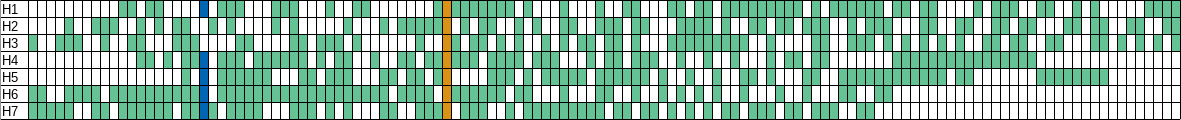
\includegraphics[width=\textwidth]{avrg_imp_rank}
        \caption{By average improvement}
        \label{fig:avrgRank}
    \end{subfigure}

    \begin{subfigure}[b]{0.95\textwidth}
        \centering
        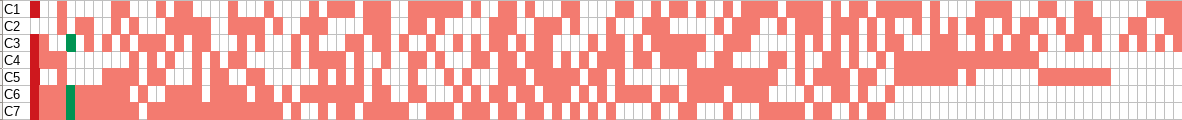
\includegraphics[width=\textwidth]{best_imp_rank}
        \caption{By best improvement}
        \label{fig:bestRank}
    \end{subfigure}

    \begin{subfigure}[b]{0.95\textwidth}
        \centering
        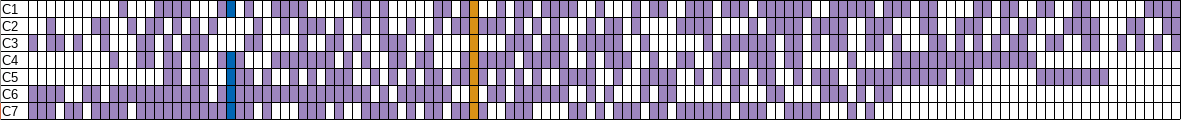
\includegraphics[width=\textwidth]{best_avrg_imp_rank}
        \caption{By best+average improvement}
        \label{fig:avrgBestRank}
    \end{subfigure}
    \label{fig:rank}
    \caption*{Highlighted tiles indicate use of a heuristic. The combinations with better results are to the left. The blue highlighted tiles show the final composition from \cref{sec:finComp}. Yellow highlighted tiles show the use of all heuristics.}
\end{figure}



\subsubsection{ANOVA and regression analysis}
The ranking gives us an overview over which heuristics are working and is always part of a good combination.
It also gives us information on which heuristics are not performing well overall and which combination of heuristics are not working well.
However, ANOVA (III) and multiple linear regression analysis can help us evaluate which heuristics have a significant positive impact on the result.
\Fref{tab:anovaNormal} shows the results of ANOVA (III) analysis performed using each heuristic as a source of variance. 
We extended the model with the instances as random effects to give us a better explanation of the result and less noise in the model. 
We did one ANOVA analysis for the average improvement over 10 runs shown in figure \ref{tab:anovaAvrgNormal}, and one for the best improvement found in figure \ref{tab:anovaBestNormal}, to see if some heuristics are making the model more robust (average) and if some heuristics are good at finding best known solutions (best). \par

\begin{table}
    \centering
    \caption{Analysis of variance}
    \begin{adjustbox}{width=\columnwidth,center}
        \begin{subtable}{.75\columnwidth}
            \centering
            \begin{tabular}{cccccc}
            \hline
            Source  &Sum sq.    &df &Mean sq.   &F      &P$>$F \\ 
            \hline
            H1      & 0.052     & 1 & 0.052     & 0.09  & 0.7682\\
            H2      & 0.748     & 1 & 0.748     & 1.26  & 0.2628\\
            H3      & 0.038     & 1 & 0.038     & 0.06  & 0.8017\\
            H4      & 22.432    & 1 & 22.432    & 37.66 & 0     \\
            H5      & 12.734    & 1 & 12.734    & 21.38 & 0     \\
            H6      & 117.945   & 1 & 117.945   & 198   & 0     \\
            H7      & 112.406   & 1 & 112.406   & 188.7 & 0     \\
            Instance& 371.704   & 4 & 92.926    & 156   & 0     \\
            Error   & 350.257   &588& 0.596     &       &       \\
            Total   & 975.207   &599&           &       &       \\
            \hline
            \end{tabular}
        \caption{Average improvement statistics}
        \label{tab:anovaAvrgNormal}
        \end{subtable}
        \hfill
        \begin{subtable}{.75\columnwidth}
            \centering
            \begin{tabular}{cccccc}
            \hline
            Source  &Sum sq.    &df &Mean sq.   &F      &P$>$F \\ 
            \hline
            H1      & 0.075     & 1 & 0.0745    & 0.23  & 0.6306\\
            H2      & 0.195     & 1 & 0.1949    & 0.61  & 0.4369\\
            H3      & 0         & 1 & 0.0001    & 0     & 0.988 \\
            H4      & 8.372     & 1 & 8.3718    & 26    & 0     \\
            H5      & 3.679     & 1 & 3.6789    & 11.43 & 0.0008\\
            H6      & 66.236    & 1 & 66.2357   & 205.71& 0     \\
            H7      & 67.081    & 1 & 67.0813   & 208.33& 0     \\
            Instance& 344.971   & 4 & 86.2428   & 267.84& 0     \\
            Error   & 189.331   &588& 0.322     &       &       \\
            Total   & 671.378   &599&           &       &       \\
            \hline
            \end{tabular}
        \caption{Best improvement statistics}
        \label{tab:anovaBestNormal}
        \end{subtable}
    \end{adjustbox}
    \label{tab:anovaNormal}
    \caption*{The columns contains in order: the source of the variability and for each source the sum of the sqares, the degrees of freedom, the mean squares, the F-statistic and the p-value.}
\end{table}

In addition to this we performed a multiple linear regression in \cref{tab:regrNormal} on the same data as the ANOVA.
The regressional analysis gives us insight into if a heuristic is positively or negatively influencing the result, aswell as how well the heuristics are explaining the result through the $R^2$.
Also here we used the instances as a random effect.

\begin{table}
    \centering
    \caption{Results of multiple linear regression model}
    \begin{adjustbox}{width=\columnwidth,center}
        \begin{subtable}{.75\columnwidth}
            \centering
            \begin{tabular}{ccccc}
            \hline
            Term    &Estimate   & SE    & tStat & pValue \\ 
            \hline                
        Intercept   & 994.58    & 0.11713       & 8491.5    & 0         \\
            H1      & -0.018582 & 0.063017      & -0.29487  & 0.7682    \\
            H2      & -0.07063  & 0.063017      & 1.1208    & 0.26283   \\
            H3      & -0.01583  & 0.063017      & -0.2512   & 0.80175   \\
            H4      & 0.39108   & 0.063729      & 6.1366    & 1.5502e-09\\
            H5      & -0.29466  & 0.063729      & -4.6236   & 4.6407e-06\\
            H6      & 0.89676   & 0.063729      & 14.071    & 5.7098e-39\\
            H7      & 0.87544   & 0.063729      & 13.737    & 1.923e-37 \\
            Inst1   & 0.50928   & 0.099639      & 5.1113    & 4.3337e-07\\
            Inst2   & -0.051052 & 0.099639      & -0.51237  & 0.60859   \\
            Inst3   & 1.6601    & 0.099639      & 16.662    & 2.4375e-51\\
            Inst4   & 1.755     &  0.099639     & 17.614    & 4.4128e-56\\
            \hline
            \end{tabular}
        \caption{Average improvement statistics, $R^2=0.641$}
        \label{tab:regrAvrgNormal}
        \end{subtable}
        \hfill
        \begin{subtable}{.75\columnwidth}
            \centering
            \begin{tabular}{cccccc}
            \hline
            Term    &Estimate   & SE    & tStat & pValue \\ 
            \hline                
        Intercept   & 994.97    & 0.086114      & 11554     & 0         \\
            H1      & 0.022291  & 0.046332      & 0.48112   & 0.63061   \\
            H2      & -0.036047 & 0.046332      & -0.77801  & 0.43687   \\
            H3      &-0.00069693& 0.046332      & -0.015042 & 0.988     \\
            H4      & 0.23891   & 0.046855      & 5.099     & 4.6112e-07\\
            H5      & -0.15838  & 0.046855      & -3.3801   & 0.00077249\\
            H6      & 0.67202   & 0.046855      & 14.342    & 3.2e-40   \\
            H7      & 0.67629   & 0.046855      & 14.434    & 1.2062e-40\\
            Inst1   & 0.64176   & 0.073257      & 8.7605    & 2.0732e-17\\
            Inst2   & 0.16783   & 0.073257      & 2.291     & 0.022316  \\
            Inst3   & 1.837     & 0.073257      & 25.077    & 6.2887e-95\\
            Inst4   & 1.6686    & 0.073257      & 22.778    & 8.2582e-83\\
            \hline
            \end{tabular}
        \caption{Best improvement statistics, $R^2=0.718$}
        \label{tab:regrBestNormal}
        \end{subtable}
    \end{adjustbox}
    \label{tab:regrNormal}
    \caption*{The columns contains in order: the term and for each term the coefficient estimate, the standard error of the coefficients, t-statistics to test if the term is significant, and the p-value}
\end{table}

\subsubsection{Observations from initial evaluation of heuristics}
Ranking the combinations in \cref{fig:rank} does indicate that using all heuristics are giving a performance in the middle of all rankings which indicates we should use a combination that excludes some heuristics. 
It also shows that H6 and H7 are usually included in the better performing combinations. \par 
The results from \cref{tab:anovaNormal} and \cref{tab:regrNormal} split our heuristics into two groups. 
The first obvious group are the significant heuristics.
The ANOVA results from table \cref{tab:anovaAvrgNormal} and \cref{tab:anovaBestNormal} tells us that four heuristics, H4-H7, have a significant impact on the result using a $95\%$ confidence interval.
However from \cref{tab:regrAvrgNormal} and \cref{tab:regrBestNormal} we see that only 3 heuristics, H4, H6 and H7, have a positive estimated coefficient, ie. a positive significant influence, for both average and best improvement (H1 is positive for best but negative for average improvement).
From this we can safely conclude that H4, H6 and H7 are significantly, positively improving the result of our model on average and they are good at finding good soolutions. 
H5 is significantly influencing the result but with a negative coefficient. 
This leads us to conclude that this heuristic either performs poorly alone, or has a negative influence on the model, to figure out which we need to do further testing.
\par
Regarding the remaining heursitics, H1, H2, and H3, we can safely conclude that they are not contributing singificantly on the result on their own, ie. an algorithm containing only these heuristics are not having a significantly positive impact on the results using a $95\%$ confidence interval.
However it could be that they have a positive effect in on the result if they are used in combination with the significant heuristics.
We therefore observe that we need further testing to know if these heuristics have a positive or negative influence on the result in combination with other heuristics.
We refer to the heuristics H1,H2,H3 and H5 as the undecided group, or G in our further evaluation of the heuristics.

\subsection{Further evaluation of heuristics}
\label{sec:evalH2}
To further analyse the performance of the heuristics we want to analyse how the heuristics are performing as an undecided group (G), see \cref{sec:evalH1}, to see if they have an effect on the results.
The result from \cref{sec:evalH1} tells us that it is out of the question to use any combination of heuristics where only heuristics from the undecided group are used.
These heuristics will alone have a negative impact on the result but it is still possible that using them combined with the significant heuristics could have a positive impact on the result
We have therefore removed the observations where the undecided group appear alone in the following testing.
We want to test if using one or several of the G heuristics in combination with other heuristics have a positive impact on the result.
We have done this in two parts.
We first wanted to see if the heuristics as a group, G, has a positive or negative influence on the result. 
To test this we have done 2-sample t-tests to compare the mean of the population where we combine the G heuristics with some significant heuristic, to the mean of the pooulation when we are not using G. 
Then we wanted to see if using G with specific combinations of the significant heuristics have significant impact on the model. 
We did this using further ANOVA (III) statistical analysis and multi linear regression model.

\subsubsection{Evaluation of undecided heuristics as a group}
The first thing we did was to run a t-test on that compares the mean of the population which include some combination of the G heuristics and the significant heuristics, towards the population that does not contain any heuristic from G. 
To represent the population without any heuristics from G we have the used the parameter $P_N$ and to represent the population with some combination of the G-heuristics and the significant heuristics we have used the parameter $P_H$.
The results from the t-test are summarized in \cref{tab:tTestGroup}.

\begin{table}
    \centering
    \caption{Results of t-tests on the undecided group mean vs no undecided heuristics}
        \begin{tabular}{ccccccc}
        \hline
                                & Improvement   &       &           &           & & Confidence\\ 
            Populations         & type          & Tail  &H-stat     & p-value   & tStat & interval \\ 
        \hline                
        $P_H-P_N$   & Average   & both  & 0 & 0.5187    & -0.6458   & -0.3785 -- 0.1912\\
        $P_H-P_N$   & Average   & right & 0 & 0.7407    & -0.6458   & -0.3326 -- inf   \\
        $P_H-P_N$   & Average   & left  & 0 & 0.2593    & -0.6458   & -inf -- 0.1453   \\
        $P_H-P_N$   & Best      & both  & 0 & 0.6903    & 0.3986    & -0.2174 -- 0.3281 \\
        $P_H-P_N$   & Best      & right & 0 & 0.3452    & 0.3986    & -0.1734 -- inf    \\
        $P_H-P_N$   & Best      & left  & 0 & 0.6548    & 0.3986    & -inf -- 0.2841    \\
       \hline
        \end{tabular}
    \caption*{The columns contain in order: the populations tested agains eachother, type of data tested(average or best improvement), tail which determines the alternative hypothesis, h-value (1 rejects the null hypothesis, 0 failure to reject), p-value of the test, t-Statistic of the test, confidence interval for the true population mean}
   \label{tab:tTestGroup}
\end{table}

We continued the testing of G by performing ANOVA (III) analysis on different combinations of the G and the significant heuristics. 
We did this to see if a combination of G and the significant heuristics could help explain the variations in the result and to see if a combination of some or all of the significant heuristics work better than others.

\begin{table}
    \centering
    \caption{Analysis of variance with the undecided group in combination with the significant heuristics}
    \begin{adjustbox}{width=\columnwidth,center}
        \begin{subtable}{.75\columnwidth}
            \centering
            \begin{tabular}{cccccc}
            \hline
            Source  &Sum sq.    &df &Mean sq.   &F      &P$>$F \\ 
            \hline
            G+H4        & 19.024    & 1 & 19.0236   & 538.34& 0     \\
            G+H6        & 0         & 1 & 0         & 0     & 0.9859\\
            G+H7        & 0.005     & 1 & 0.0045    & 0.13  & 0.7204\\
            G+H4+H6     & 0.059     & 1 & 0.0589    & 1.67  & 0.1973\\
            G+H4+H7     & 0.001     & 1 & 0.0009    & 0.03  & 0.8722\\
            G+H6+H7     & 0.22      & 1 & 0.2202    & 6.23  & 0.0128\\
            G+H4+H6+H7  & 0.166     & 1 & 0.1657    & 4.69  & 0.0308\\
            Inst        & 309.022   & 4 & 77.2555   &2186.21& 0     \\
            Error       & 19.365    &548& 0.0353    &       &       \\
            Total       & 385.274   &559&           &       &       \\
            \hline
            \end{tabular}
        \caption{Average improvement statistics}
        \label{tab:anovaAvrgGroup}
        \end{subtable}
        \hfill
        \begin{subtable}{.85\columnwidth}
            \centering
            \begin{tabular}{cccccc}
            \hline
            Source  &Sum sq.    &df &Mean sq.   &F      &P$>$F \\ 
            \hline
            G+H4        & 12.879    & 1 & 12.8793   & 609.42& 0     \\
            G+H6        & 0.131     & 1 & 0.1307    & 6.19  & 0.0132\\
            G+H7        & 0.239     & 1 & 0.2389    & 11.31 & 0.0008\\
            G+H4+H6     & 0.223     & 1 & 0.2227    & 10.54 & 0.0012\\
            G+H4+H7     & 0.153     & 1 & 0.1525    & 7.22  & 0.0074\\
            G+H6+H7     & 0.42      & 1 & 0.4195    & 19.85 & 0     \\
            G+H4+H6+H7  & 0.395     & 1 & 0.395     & 18.69 & 0     \\
            Inst        & 295.738   & 4 & 73.9346   &3498.45& 0     \\
            Error       & 11.581    &548& 0.0211    &       &       \\
            Total       & 352.547   &559&           &       &       \\
            \hline
            \end{tabular}
        \caption{Best improvement statistics}
            \label{tab:anovaBestGroup}
        \end{subtable}
    \end{adjustbox}
    \label{tab:anovaGroup}
    \caption*{The columns contains in order: the source of the variability and for each source the sum of the sqares, the degrees of freedom, the mean squares, the F-statistic and the p-value.}
\end{table}

The results are summarized in table \ref{tab:anovaGroup} and \cref{tab:regrGroup}. 
As an example a source of G+H4, contains all observations where at least one of the undecided heuristics from G are combined exclusively with H4.

\begin{table}
    \centering
    \caption{Results of multiple linear regression model with the undecided group in combination with the significant heuristics}
    \begin{adjustbox}{width=\columnwidth,center}
        \begin{subtable}{.95\columnwidth}
            \centering
            \begin{tabular}{ccccc}
            \hline
            Term    &Estimate   & SE    & tStat & pValue \\ 
            \hline                
        Intercept       & 995.85    & 0.035525      & 28032     & 0         \\
            G+H4        & -0.89285  & 0.038481      & -23.202   & 1.8003e-83\\
            G+H6        & 0.00068095& 0.038481      & 0.017696  & 0.98589   \\
            G+H7        & 0.013782  & 0.038481      & 0.35815   & 0.72037   \\
            G+H4+H6     & 0.049672  & 0.038481      & 1.2908    & 0.19731   \\
            G+H4+H7     & -0.0061945& 0.038481      & -0.16097  & 0.87217   \\
            G+H6+H7     & 0.096062  & 0.038481      & 2.4963    & 0.012841  \\
            G+H4+H6+H7  & 0.083317  & 0.038481      & 2.1651    & 0.030808  \\
            Inst1       & 0.53458   & 0.02512       & 21.281    & 1.0604e-73\\
            Inst2       & 0.031671  & 0.02512       & 1.2608    & 0.20793   \\
            Inst3       & 1.71      & 0.02512       & 68.073    &1.6221e-269\\
            Inst4       & 1.5959    & 0.02512       & 63.531    &6.3233e-255\\
            \hline
            \end{tabular}
        \caption{Average improvement statistics, $R^2=0.95$}
        \label{tab:regrAvrgGroup}
        \end{subtable}
        \hfill
        \begin{subtable}{.75\columnwidth}
            \centering
            \begin{tabular}{cccccc}
            \hline
            Term    &Estimate   & SE    & tStat & pValue \\ 
            \hline                
        Intercept       & 995.88    & 0.027473      & 36249     & 0         \\
            G+H4        & -0.73464  & 0.029759      & -24.686   & 5.012e-91 \\
            G+H6        & 0.07402   & 0.029759      & 2.4873    & 0.013167  \\
            G+H7        & 0.10006   & 0.029759      & 3.3625    & 0.00082635\\
            G+H4+H6     & 0.096599  & 0.029759      & 3.246     & 0.0012417 \\
            G+H4+H7     & 0.079948  & 0.029759      & 2.6865    & 0.0074396 \\
            G+H6+H7     & 0.13259   & 0.029759      & 4.4554    & 1.0157e-05\\
            G+H4+H6+H7  & 0.12865   & 0.029759      & 4.3232    & 1.8269e-05\\
            Inst1       & 0.70773   & 0.019426      & 36.432    &1.6371e-148\\
            Inst2       & 0.27728   & 0.019426      & 14.273    & 1.5823e-39\\
            Inst3       & 1.873     & 0.019426      & 96.415    & 0         \\
            Inst4       & 1.5781    & 0.019426      & 81.237    &8.6749e-308\\
            \hline
            \end{tabular}
        \caption{Best improvement statistics, $R^2=0.967$}
        \label{tab:regrBestGroup}
        \end{subtable}
    \end{adjustbox}
    \label{tab:regrGroup}
    \caption*{The columns contains in order: the term and for each term the coefficient estimate, the standard error of the coefficients, t-statistics to test if the term is significant, and the p-value}
\end{table}

\subsubsection{Observations from results of the heuristics further evaluation}
The results from \cref{tab:tTestGroup} tells us that we cannot reject the null hypothesis, for all populations, that the mean of the two populations are different using a $95\%$ confidence interval. This is the case for both average and best improvement.
This tells us that the heuristics from the undecided group (G) either have no significant impact on the result, or that the effect from some are nulling out the others. Further testing is needed to make any further conclusions. \par
Table \ref{tab:anovaGroup} and \cref{tab:regrGroup} gives us further insight into our model.
First of all the result from \cref{tab:anovaAvrgGroup} tells us that only two combinations of the undecided group and the significant variables have a significant impact on the result using a $95\%$ confidence interval.
Using some heuristics from the undecided group combined with heuristic H6 and H7, aswell as H4 has a significant impact on the average improvement result.
From \cref{tab:regrAvrgGroup} we also see that the combinations are also getting a positive coefficient.
We also observe that the $R^2 = 0.95$ is very high so this model explains the results very well and this supports the use of these heuristic combination in regards to the average improvement.
\par
The same combinations are significant and positive in reagards to the best improvement tabels \cref{tab:anovaBestGroup} and \cref{tab:regrBestGroup}.
And even though more combinations are significant for best improvement, the combinations with highest positive estimated coefficients are still including H6 and H7, or H6 H7 and H4.
We also observe here the increased $R^2 = 0.967$ which indicates that this model is explaining the result from best and average improvement very well.
This could indicate that the conmbinations with H6, H7 and H4 are consistently contributing to the same positive results.
\par
The results from the further testing tells us that there are combinations of the undecided group and the significant heuristics that have a positive significant impact on the result of both average and best improvement. 
It supports our results from \cref{sec:evalH1} of significant heuristics H6, H7 and H4 and leads us to conclude that there might be a positive influence from the undecided group heuristics, however further testing is nessecary to determine which heuristics should be included. 

\subsection{Evaluation of individual heuristics}
\label{sec:evalI}
Until now, the heuristic H4, H6 and H7 have been proven significant.
The heuristics H1, H2, H3 and H5 have been proven significant in combination with the significant heuristics but not alone.
We continue refering to them as the undecided group heuristics or G. 
\par
We want to figure out which of the heuristics in the undecided group, if any, have a positive, or negative, influence on the result.
To do this we performed pairwise t-tests to check if an undecided heuristic is significantly improving or decreasing the best and average improvement.
Like in \cref{sec:evalH2} it is out of the question to use any combination of heuristics where only undecided heuristics are used, so we remove these observations from the data also in these tests.
In our tests we test if the mean of the populations where we combine the undecided heuristics with some significant heuristic is significantly different than the population when we are not using an undecided heuristic. 

\subsubsection{T-tests of individual heuristics}
Similar to the previous section we use the parameter $P^{H_i}_{NA}$ to refer to the population without a specific heuristic $H_i$ for the average improvement, indicated by $A$, and the parameter $P^{H_i}_{HB}$ as the population including the heuristic $H_i$ for the best improvement, indicated by $B$. 
Here $H_i$ represents one of the heuristics described in the previous section. 
We did the test for all 4 of the undecided heuristics from the previous section $H_1$, $H_2$, $H_3$ and $H_5$.
The results from the pairwise t-tests are summarized in \cref{tab:tTest}.

\begin{table}
    \centering
    \caption{Results of t-tests on individual heuristics}
        \begin{tabular}{ccccccc}
        \hline
            Populations                 & Tail   &H-stat   & p-value    & tStat & conf-int \\ 
        \hline                
            $P^{H_1}_{HA}-P^{H_1}_{NA}$    & both  & 0 & 0.5427    & -0.6090  & -0.1580 -- 0.0727 \\
            $P^{H_1}_{HA}-P^{H_1}_{NA}$    & right & 0 & 0.7286    & -0.6090  & -0.1325 -- inf    \\
            $P^{H_1}_{HA}-P^{H_1}_{NA}$    & left  & 0 & 0.2714    & -0.6090  & -inf -- 0.0472    \\
            $P^{H_1}_{HB}-P^{H_1}_{NB}$    & both  & 0 & 0.9240    & -0.0955  & -0.1428 -- 0.1296 \\
            $P^{H_1}_{HB}-P^{H_1}_{NB}$    & right & 0 & 0.5380    & -0.0955  & -0.1208 -- inf    \\
            $P^{H_1}_{HB}-P^{H_1}_{NB}$    & left  & 0 & 0.1076    & -0.0955  & -inf -- 0.1076    \\
            $P^{H_2}_{HA}-P^{H_2}_{NA}$    & both  & 1 & 3.4853e-10& -6.5098  & -0.0692 -- 0.0412 \\
            $P^{H_2}_{HA}-P^{H_2}_{NA}$    & right & 0 & 1.0000    & -6.5098  & -0.0661 -- inf    \\
            $P^{H_2}_{HA}-P^{H_2}_{NA}$    & left  & 1 & 1.7426e-10& -6.5098  & -inf -- 0.0443    \\
            $P^{H_2}_{HB}-P^{H_2}_{NB}$    & both  & 1 & 4.5425e-10& -3.5486  & -0.0370 -- 0.0106 \\
            $P^{H_2}_{HB}-P^{H_2}_{NB}$    & right & 0 & 0.9998    & -3.5486  & -0.0349 -- inf    \\
            $P^{H_2}_{HB}-P^{H_2}_{NB}$    & left  & 1 & 2.2712e-04& -3.5486  & -inf -- 0.0127    \\
            $P^{H_3}_{HA}-P^{H_3}_{NA}$    & both  & 1 & 0.0244    & -2.2635  & -0.0276 -- -0.0043\\
            $P^{H_3}_{HA}-P^{H_3}_{NA}$    & right & 0 & 0.9878    & -2.2635  & -0.0250 -- inf    \\
            $P^{H_3}_{HA}-P^{H_3}_{NA}$    & left  & 1 & 0.0122    & -2.2635  & -inf -- -0.0069  \\
            $P^{H_3}_{HB}-P^{H_3}_{NB}$    & both  & 0 & 0.6271    & -0.4864  & -0.0134 -- 0.0081  \\
            $P^{H_3}_{HB}-P^{H_3}_{NB}$    & right & 0 & 0.6865    & -0.4864  & -0.0116 -- inf     \\
            $P^{H_3}_{HB}-P^{H_3}_{NB}$    & left  & 0 & 0.3135    & -0.4864  & -inf -- 0.0063     \\
            $P^{H_5}_{HA}-P^{H_5}_{NA}$    & both  & 0 & 0.4702    & -0.7231  & -0.0301 -- 0.0118  \\
            $P^{H_5}_{HA}-P^{H_5}_{NA}$    & right & 0 & 0.7649    & -0.7231  & -0.0255 -- inf     \\
            $P^{H_5}_{HA}-P^{H_5}_{NA}$    & left  & 0 & 0.2351    & -0.7231  & -inf -- 0.0071     \\
            $P^{H_5}_{HB}-P^{H_5}_{NB}$    & both  & 1 & 1.7956e-04& -3.7972  & -0.0167 -- 0.0528  \\
            $P^{H_5}_{HB}-P^{H_5}_{NB}$    & right & 1 & 8.9779e-05& -3.7972  & -0.0197 -- inf     \\
            $P^{H_5}_{HB}-P^{H_5}_{NB}$    & left  & 0 & 0.9999    & -3.7972  & -inf -- 0.0499     \\
        \hline
        \end{tabular}
    \caption*{The columns contain in order: the populations tested agains eachother, type of data tested(average or best improvement), tail which determines the alternative hypothesis, h-value (1 rejects the null hypothesis, 0 failure to reject), p-value of the test, t-Statistic of the test, confidence interval for the true population mean}
   \label{tab:tTest}
\end{table}

\subsubsection{Observations from the results of the individual heuristic evaluations}
The first thing we see from the t-tests is that the effect of the heuristics are cancelling eachother out, as some are left significant, and some are right significant.
We go through each of the heuristics results from \cref{tab:tTest} here. \par
For the heuristic H1 the population mean of both best and average improvement is not significantly different using a $95\%$ confidence interval. It follows then that the tails are also not significantly different. \par
Regarding the results for heuristic H2 we reject the null hypothesis that the means are equal using a $95\%$ significanse interval for the average and best improvement regarding this heuristic. 
The left tail alternative hypothesis' that the means of $P^{H_2}_{HA}$ and $P^{H_2}_{HB}$ is lower than $P^{H_2}_{NA}$ and $P^{H_2}_{NB}$ are accepted, while the right tail alternative hypothesis is rejected for both best and average improvement.\par 
The results of H3 show that the null hypothesis that the population mean of $P^{H_3}_{HA}$ is equal to the population mean of $P^{H_3}_{NA}$ is rejected and accepted for $P^{H_3}_{HB}$ and $P^{H_3}_{NB}$. The left tail alternative hypothesis that the means of $P^{H_3}_{HA}$ is with $95\%$ confidence lower than $P^{H_3}_{NA}$ , is accepted.\par 
For H5 the null hypothesis is rejected for  $P^{H_5}_{HB}$ and  $P^{H_5}_{NB}$ and accepted for $P^{H_5}_{HA}$ and $P^{H_5}_{NA}$ . 
The alternative hypothesis of the right tail of the best improvement, that the mean is significantly higher in $P^{H_5}_{HB}$ than  $P^{H_5}_{NB}$ is accepted.

The results summarized above tells us that using H1 will have no effect on the outcome of the result. 
Also H2 and H3 are significantly decreasing the average for both heuristics and also for best for H2. 
This indicates that it is not beneficial to include these heuristics in a model.
Finally H5 is not affecting the average improvement however it is positively effecting the best improvement, indicating that it could be beneficial to include this heuristic.

\subsection{Deciding on the final model composition}
\label{sec:finComp}
The results from \cref{sec:wild} tells us that our final model should include our wild algorithm. 
This will influence our running time a little but give us much more reliable results.
\par
As for selecting heuristics to include, the results from section \cref{sec:evalH1} and \cref{sec:evalH2}, indicates that we need to include H4, H6 and H7 in our final model.
We observed from our testing of the wild algorithm that the running time of H1 is significantly lower than our other heuristics \cref{fig:wildRes}. Even though \cref{sec:evalI} showed us that H1 had no significant effect on the model, the low running time is leading us to rather include this heuristic than not, to lower the running time of our algorithm overall.
It will as \cref{sec:evalI} also showed have no significant negative effect on the results of our model.
H5 is also not effecting the average improvement of our model but it significantly effects the result of the best improvement found. This tells us that we should include this heuristic in our final composition. \par
The results from \cref{sec:evalH2} indicated that a combination of H4, H6 and H7 + some of combination of the undecided group heuristics is significantly effecting both the average and best improvement. Therefore our final model composition will be the ALNS algorithm with the wild algorithm and heuristics H1, H4, H5, H6 and H7.

\section{Final results}
\label{sec:evalFin}
After deciding on a model best suited to our problem we did a final run of our algorithm using composition described in the previous section.
The algorithm was run using 5 instance sets of each 5 representative sizes. 
\subsection{Evaluation of final model}
\label{sec:finRes}
For each instance we used the powerful maschine to let AMPL try for 10 000 seconds to find an optimal solution for each instance. 
The larger runs resulted in a "out of memory" failure message so these results we simply marked as NA.
The results from the runs of our final model composition together with the mathematical model runs in AMPL are summarized in \cref{tab:finRes}. 

\begin{table}
    \centering
    \caption{Model performance in european instance set 1}
    \begin{adjustbox}{width=0.95\columnwidth,center}
            \begin{tabular}{|cccc|ccc|ccc|c|}
                \hline
                    &    &       &       & \multicolumn{3}{c}{Mathematical model}    & \multicolumn{3}{|c|}{SCALNS}                & \\
                \hline
                    Inst&           &       &       & Solution      & Optimaily     & Run       & Average       & Best      & Avrg run      &              \\ 
                    Set & #Ord      & #Veh  & #Loc  & objective     & gap           & time(sec) & objective     & objective & Time          & delta        \\ 
            \hline
                \multirow{5}{*}{\begin{sideways} Set 1 \end{sideways}}  
                        & 4       & 3     & 7     & $3\,444.7$      & $0.00\%$      & 0.1       & $3\,444.7$    & $3\,444.7$    & $0.1$     & $0.00\%$  \\
                        & 12      & 7     & 9     & $149\,692.3$    & $0.00\%$      & 9963.7    & $149\,692.4$  & $149\,692.3$  & $0.5$     & $0.00\%$  \\
                        & 35      & 20    & 22    & $2\,091\,776.5$ & $99.91\%$     & 10000.2   & $10\,323.2$   & $9\,997.9$    & $2.8$     & $99.52\%$  \\
                        & 80      & 45    & 45    & $6\,422\,128.6$ & $99.99\%$     & 10000.0   & $21\,170.5$   & $20\,911.5$   & $21.1$    & $99.67\%$  \\
                        & 150     & 80    & 85    & NA              & NA            & NA        & $34\,479.1$   & $32\,798.0$   & $100.8$   & NA  \\
            \hline
                \multirow{5}{*}{\begin{sideways} Set 2 \end{sideways}}  
                        & 4       & 3     & 7     & $2\,501.0$      & $0.00\%$      & 0.1       & $2\,501.0$    & $2\,501.0$    & $0.1$     & $0.00\%$  \\
                        & 12      & 7     & 9     & $5\,987.8$      & $0.00\%$      & 1041.8    & $5\,987.8$    & $5\,987.8$    & $0.6$     & $0.00\%$  \\
                        & 35      & 20    & 22    & $1\,985\,165.5$ & $99.90\%$     & 10000.3   & $14\,382.4$   & $14\,272.1$   & $2.6$     & $99.28\%$  \\
                        & 80      & 45    & 45    & $6\,809\,899.5$ & $99.99\%$     & 10000.0   & $25\,736.6$   & $24\,760.8$   & $16.8$    & $99.64\%$  \\
                        & 150     & 80    & 85    & NA              & NA            & NA        & $36\,927.2$   & $35\,932.1$   & $112.1$   & NA  \\
            \hline
                \multirow{5}{*}{\begin{sideways} Set 3 \end{sideways}}  
                        & 4       & 3     & 7     & $1\,404.0$      & $0.00\%$      & 0.3       & $1\,404.0$    & $1\,404.0$    & $0.1$     & $0.00\%$  \\
                        & 12      & 7     & 9     & $5\,862.5$      & $33.16\%$     & 10000.0   & $5\,862.5$    & $5\,862.5$    & $0.9$     & $0.00\%$  \\
                        & 35      & 20    & 22    & $679\,594.8$    & $99.71\%$     & 10000.4   & $6\,334.7$    & $6\,267.7$    & $3.7$     & $99.08\%$  \\
                        & 80      & 45    & 45    & $5\,748\,613.6$ & $99.99\%$     & 10000.5   & $12\,609.0$   & $12\,347.6$   & $32.2$    & $99.79\%$  \\
                        & 150     & 80    & 85    & NA              & NA            & NA        & $19\,771.9$   & $19\,149.8$   & $126.1$   & NA  \\
            \hline
                \multirow{5}{*}{\begin{sideways} Set 4 \end{sideways}}  
                        & 4       & 3     & 7     & $1\,696.1$      & $0.00\%$      & 0.7       & $1\,696.1$    & $1\,696.1$    & $0.1$     & $0.00\%$  \\
                        & 12      & 7     & 9     & $3\,285.2$      & $21.45\%$     & 10000.0   & $3\,109.6$    & $3\,109.6$    & $1.5$     & $5.35\%$  \\
                        & 35      & 20    & 22    & $547\,881.6$    & $99.72\%$     & 10000.2   & $4\,652.8$    & $4\,494.5$    & $5.1$     & $99.18\%$  \\
                        & 80      & 45    & 45    & $6\,201\,301.5$ & $99.99\%$     & 10000.1   & $15\,540.0$   & $15\,290.6$   & $21.4$    & $99.75\%$  \\
                        & 150     & 80    & 85    & NA              & NA            & NA        & $22\,508.6$   & $22\,252.6$   & $103.4$   & NA  \\
            \hline
                \multirow{5}{*}{\begin{sideways} Set 5 \end{sideways}}  
                        & 4       & 3     & 7     & $5\,154.9$      & $0.00\%$      & 0.4       & $5\,154.9$    & $5\,154.9$    & $0.1$     & $0.00\%$  \\
                        & 12      & 7     & 9     & $3\,716.2$      & $22.93\%$     & 10000.2   & $3\,716.2$    & $3\,716.2$    & $0.6$     & $0.00\%$  \\
                        & 35      & 20    & 22    & $1\,757\,079.6$ & $99.90\%$     & 10000.2   & $13\,138.9$   & $12\,944.2$   & $2.1$     & $99.26\%$  \\
                        & 80      & 45    & 45    & $5\,909\,616.9$ & $99.99\%$    & 10000.0   & $24\,034.0$   & $23\,855.5$   & $9.1$     & $99.60\%$  \\
                        & 150     & 80    & 85    & NA              & NA            & NA        & $41\,343.4$   & $39\,847.0$   & $82.6$    & NA  \\
            \hline
            \end{tabular}
    \end{adjustbox}
    \label{tab:finRes}
    \caption*{The columns contains in order:Instance set, number of orders, number of vehicles and number of locations in the instances. 
    The next three columns contain the result from running our mathematical model (MM) run in AMPL; solution objective, optimality gap and the running time.
    Then follows 3 columns with the results of our model, average objective found, best objective found and average running time. 
    The final column contains a delta which is calculated as follows: (solution objective MM - SCALNS best objective)/solution objective MM.}
\end{table}

\Cref{fig:heuristics} shows the weight of each heuristic through each segment of our model SCALNS segments for arbitrarily selected runs. 
The vertical blue lines indicate which segment the best solution for the current run was found. The most relevant sections are the ones before this blue lines.

\begin{figure}
    \centering
    \caption{Operator weights per segment from instance set 1}
    \begin{subfigure}[b]{0.45\textwidth}
        \centering
        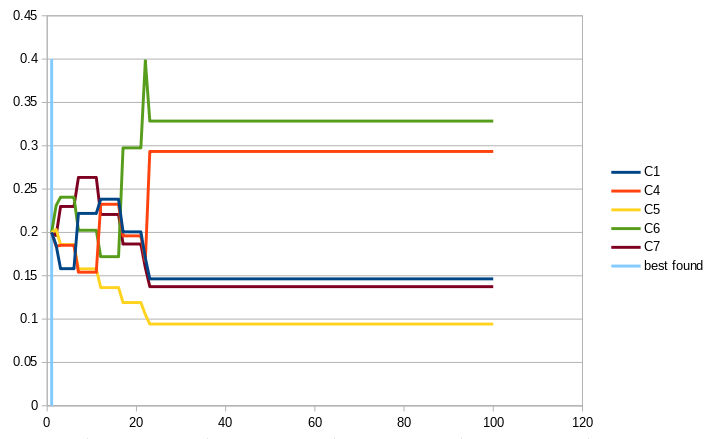
\includegraphics[width=\textwidth]{operators_4_ord}
        \caption{Instance size 4 orders, run 1}
        \label{fig:operators4}
    \end{subfigure}
    \hfill
    \begin{subfigure}[b]{0.45\textwidth}
        \centering
        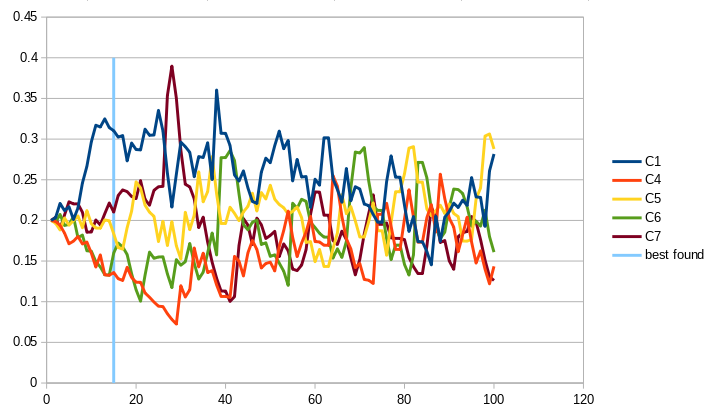
\includegraphics[width=\textwidth]{operators_12_ord}
        \caption{Instance size 12 orders, run 3}
        \label{fig:operators12}
    \end{subfigure}

    \begin{subfigure}[b]{0.45\textwidth}
        \centering
        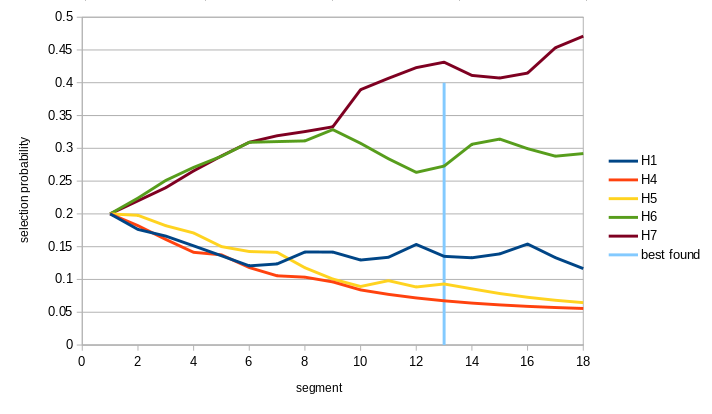
\includegraphics[width=\textwidth]{operators_35_ord}
        \caption{Instance size 35 orders, run 5}
        \label{fig:operators35}
    \end{subfigure}
    \hfill
    \begin{subfigure}[b]{0.45\textwidth}
        \centering
        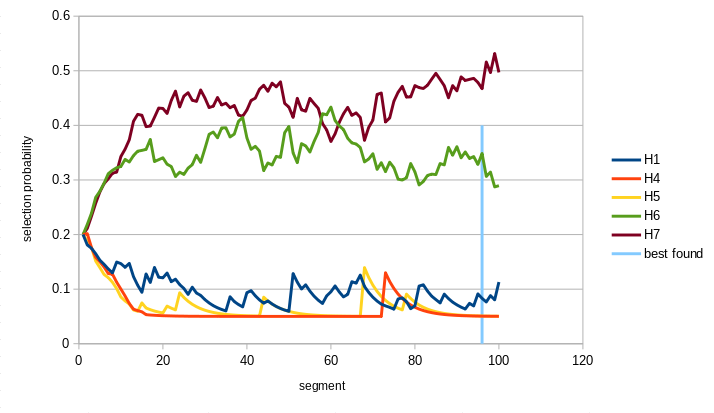
\includegraphics[width=\textwidth]{operators_80_ord}
        \caption{Instance size 80 orders, run 7}
        \label{fig:operators80}
    \end{subfigure}

    \begin{subfigure}[b]{0.45\textwidth}
        \centering
        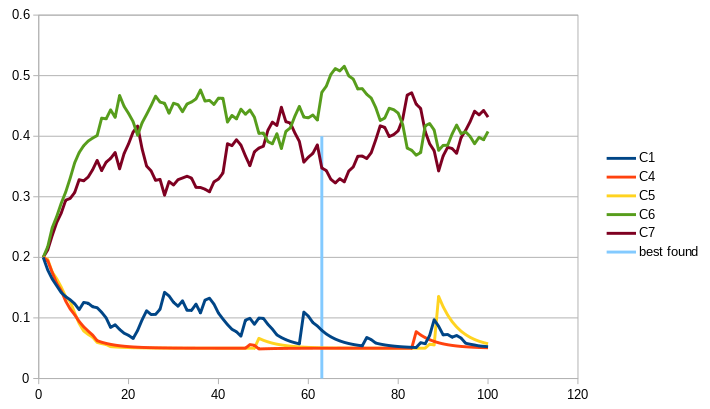
\includegraphics[width=\textwidth]{operators_150_ord}
        \caption{Instance size 150 orders, run 9}
        \label{fig:operators150}
    \end{subfigure}
    \label{fig:heuristics}
    \caption*{The y-axis represent the weight of each heuristic, the x-axis represent a segment run. The blue vertical lines represent the segment where the best solution was found.}
\end{figure}


\subsection{Observations of results  the final composition}
\label{sec:finalObs}
The first noticeable thing from the results of \cref{tab:finRes} is that the performance of the mathematical model is quickly deteriarating with the size of the instances.
Already at the second instance size the model is struggeling to finish on time, and for set 3 and set 5 there is still an optimality gap.
For the third instance size (35 orders) the model can barely start iterating through solutions and the solution objecteve after 10 000 seconds has a very large optimality gap. 
We observe that the optimality gap is very large for the third and fourth instance size (35 orders and 80 orders) which means that the AMPL would need substantially more that 10 000 seconds to search for any type of real solution.
This tells us that our problem is quickly getting very complex and that building a good model that can quickly find close to optimal solutions would be very important for this problem.
\par
Moving on to the results of our SCALNS model, there are several observations that are important here. 
We see from the smallest instance size (4 orders) that our model is performing equally with the Mathematical model in terms of optimal solution but is already beating it in terms of running time.
This is not unexpected as the smallest problem does not require a lot of iterations but it is unexpected that our model beats the mathematical model quite consistently in terms of running time.
\par
As we increase the instance size to 12 orders, we see that our model consistently finds the same solution as AMPL, apart for in one case (instance 4) where AMPL was not able to find the optimal solution in 10 000 seconds.
This combined with the fact that our model is doing this in around 1 second for this instances of this size tells us that our model is performing very well.
It is also showing that our model is a robust model as the average and best solutions found are all the same for instances of size orders $\leq12$.
\par
For the larger instance sizes (orders $\geq35$) AMPL was not able to find any solutions remotely close to the optimal value. The delta from \cref{fig:finRes} is higher than $99\%$ for all these instances, which indicates that our model is significantly faster and better at finding good solutions.
Another observation is how tight the best solution is overall with the average solution, also for the larger instance sets. 
This further indicates that our model is very robust and consistently finding similar solutions.
A best solution much lower than the average could indicate that our model cannot move away from a local optimum in some cases.
However our average solutions are within a $5\%$ range of the best solutions.
This means we are consistently hitting solutions close to the best known.
\par
The \cref{fig:heuristics} show the performance of our heuristics.
\Cref{fig:operators12} show that for smaller instances the heuristics H1, H5 aswell as H7 are getting higher weights before we find the optimal solution. This indicates that they are important for the smaller instances.
The remaining figures \ref{fig:operators35}, \ref{fig:operators80} and \ref{fig:operators150} indicate that H6 and H7 are the most important heuristics that our algorithm are giving more weight than the others and that they are consistently outperforming the other heuristics in regards to finding new and better solutions. 
We do however see several spikes from the heuristic H5 and H1 up until the best solution is found (blue line). 
Which indicate that they are contributing on possibly moving to new and/or better solutions from time to time. 
The H1, H5, and H4 are doing this less consistently than H6 an H7 for larger instance sets, but that doesnt mean that they are not important for the final result. \par
These observations also support our observations from \cref{sec:evalH1} and \cref{sec:evalH2}, where H6 and H7 are outperforming the other heuristics. 
Another observation from \cref{tab:finRes} is that clearly our adaptive weights are important for our search as size and problem constraints influence how the heuristics are performing and thereby changing how our model gives them weight. 

\biblio                                                         
\end{document}  
